\documentclass[conference]{IEEEtran}
\usepackage{cite}
\usepackage{amsmath,amssymb}
\usepackage{graphicx}
\usepackage{booktabs}
\usepackage{textcomp}
\usepackage[font=footnotesize,labelsep=period]{caption}
\captionsetup[table]{justification=raggedright,singlelinecheck=false}
\newcommand{\ev}[2]{#2}
\newcommand{\mf}{macro-F\textsubscript{1}}
\newcommand{\mi}{micro-F\textsubscript{1}}
\newcommand{\tablegap}{\setlength{\tabcolsep}{4pt}}
\usepackage[utf8]{inputenc}
\usepackage[T5]{fontenc}
\usepackage[vietnamese]{babel}
\renewcommand{\IEEEkeywordsname}{Từ khóa}
\begin{document}
\title{Nhận diện cảm xúc theo ngữ cảnh có giải thích, dẫn dắt bằng văn bản và suy luận chuỗi}
\author{\IEEEauthorblockN{N. Q. Sang}
\IEEEauthorblockA{Trí tuệ nhân tạo, Đại học FPT\\
sangquang2904@gmail.com}}
\maketitle

\begin{abstract}
Mô tả bằng văn bản tạo ra một biểu diễn có thể kiểm tra được cho bài toán nhận diện cảm xúc theo ngữ cảnh, nhưng lời giải thích lưu loát chưa chắc phản ánh hành vi của bộ phân loại. Chúng tôi nghiên cứu trên EMOTIC một chuỗi xử lý theo giai đoạn, gồm trích xuất dấu hiệu nhìn thấy được, phân loại đa nhãn, can thiệp theo phương thức và giải thích bằng lời. Các bộ mã hóa văn bản và thị giác được đóng băng cung cấp đầu vào cho các Transformer ngữ nghĩa và đa phương thức có thể huấn luyện. Với các seed 42--44, mô hình đầy đủ đạt mAP trung bình trên test là 30.10 và \mf{} là 33.90, so với 27.15 và 31.59 của biến thể chỉ dùng thị giác, và 27.35 và 30.94 của baseline ResNet-50 được huấn luyện tốt nhất. Khoảng bootstrap ghép cặp theo ảnh không chứa giá trị không ở mọi seed khi so với biến thể chỉ dùng thị giác và cả ba baseline ResNet-50. Bỏ dấu hiệu về người làm mAP test giảm còn 28.49, trong khi bỏ một token thị giác, bỏ dấu hiệu ngữ cảnh hoặc xóa một tập từ cảm xúc cố định chỉ làm thay đổi dưới một điểm. Lời giải thích từ checkpoint ở seed 42 có 99.92\% lượt trích số khớp với một giá trị được phép trong bằng chứng, nhưng nêu luồng người ở 7149 trên 7184 phản hồi test dùng được và chỉ khớp với phương thức gây giảm điểm lớn nhất ở 31.83\%, thấp hơn 51.00\% của mốc tham chiếu luôn nêu phương thức phổ biến nhất. Các kết quả này phân biệt lợi ích dự đoán của dấu hiệu văn bản với tính trung thực còn hạn chế của lời giải thích. Các thí nghiệm không so sánh suy luận chuỗi (chain-of-thought, tức suy luận từng bước) với trả lời trực tiếp.
\end{abstract}
\begin{IEEEkeywords}
nhận diện cảm xúc theo ngữ cảnh, dấu hiệu bằng văn bản, học đa phương thức, tính trung thực của lời giải thích, EMOTIC
\end{IEEEkeywords}

\section{Giới thiệu}\label{sec:introduction}
Nhận diện cảm xúc trong ảnh tự nhiên hướng đến cảm xúc biểu hiện ra bên ngoài của một người, chứ không cho phép tiếp cận trực tiếp trạng thái tâm lý bên trong. EMOTIC kết hợp chú thích về người với thông tin cảnh để dự đoán các loại cảm xúc \cite{emotic}. Các mạng có xét ngữ cảnh kết hợp đặc trưng của người và môi trường \cite{caer}, còn EmotiCon nghiên cứu những cách diễn giải ngữ cảnh bổ trợ cho nhau \cite{emoticon}. Những hướng tiếp cận này thúc đẩy việc xem xét đóng góp của người mục tiêu, ảnh xung quanh và mô tả bằng văn bản đối với nhận diện.

Mô hình thị giác--ngôn ngữ có thể mô tả tư thế, hành động, đồ vật và tương tác bằng ngôn ngữ thông thường. Các mô tả thể hiện thông tin mà người phân tích có thể kiểm tra và một bộ phân loại riêng có thể sử dụng. Ước lượng cảm xúc từ chú thích ảnh \cite{captions} và mô tả tự sự cho lý thuyết tâm trí về cảm xúc \cite{etom} là những tiền đề liên quan. Tuy nhiên, khả năng kiểm tra biểu diễn chưa đủ để khẳng định rằng lời giải thích được tạo sau đó phản ánh trung thực cách bộ phân loại đã sử dụng biểu diễn ấy.

Trong tiêu đề, \emph{dẫn dắt bằng văn bản và suy luận chuỗi} được hiểu theo cách vận hành của hệ thống: dấu hiệu nhìn thấy được được diễn đạt thành văn bản; bộ phân loại kết hợp đặc trưng văn bản và thị giác; các can thiệp tạo bằng chứng về độ nhạy theo phương thức; mô hình ngôn ngữ diễn đạt lại bằng chứng đó. Đây là chuỗi tính toán theo giai đoạn, không phải khẳng định rằng văn bản bộc lộ dấu vết suy luận bên trong. Prompt suy luận chuỗi, vốn gợi ra các bước suy luận trung gian \cite{cot}, là một nguồn động lực có liên quan; các thí nghiệm hiện tại không so sánh kỹ thuật suy luận chuỗi với trả lời trực tiếp. Lời giải thích được tạo sau bước phân loại và không quyết định các nhãn của bước này.

Chúng tôi đặt câu hỏi liệu văn bản có cải thiện bộ phân loại thị giác tương ứng hay không, mô hình hợp nhất phụ thuộc vào những luồng văn bản và thị giác nào, và liệu lời giải thích có xác định được phương thức mà bộ phân loại nhạy nhất hay không. Đóng góp là triển khai và phân tích thực nghiệm chuỗi xử lý này, tách lợi ích dự đoán khỏi hành vi giải thích. Chúng tôi báo cáo bảy biến thể được huấn luyện lại với ba seed, so sánh chúng với ba baseline ResNet-50 được huấn luyện, phân biệt biến thiên giữa các seed với độ bất định do lấy mẫu ảnh, và so sánh lời giải thích với mốc tham chiếu hằng số cùng mốc tham chiếu suy ra từ can thiệp. Dấu hiệu văn bản, đặc biệt là dấu hiệu về người, mang giá trị dự đoán nhất quán, nhưng lời giải thích không xác định được luồng thông tin quan trọng. Chúng tôi không khẳng định đạt kết quả tốt nhất hiện nay hay chứng minh khả năng suy luận nhân quả.

\section{Nghiên cứu liên quan}\label{sec:related}
\subsection{Nhận diện từ thị giác và ngữ cảnh}
EMOTIC nghiên cứu cảm xúc biểu hiện ra bên ngoài dựa trên thông tin về người và ngữ cảnh \cite{emotic}. CAER-Net mã hóa riêng khuôn mặt và ngữ cảnh, rồi kết hợp thích nghi các đặc trưng \cite{caer}. EmotiCon đưa vào ngữ cảnh đa phương thức, ngữ nghĩa và tương tác \cite{emoticon}. ARBEE phát triển dữ liệu và mô hình hóa cảm xúc được cảm nhận từ chuyển động cơ thể \cite{arbee}, còn EmotionCLIP học biểu diễn từ giao tiếp bằng lời và phi ngôn ngữ \cite{emotionclip}. Các công trình này gợi ý những nguồn thông tin bổ trợ, nhưng không xác lập lợi ích của chúng đối với cách triển khai của chúng tôi.

Ngữ cảnh có thể tạo ra các liên hệ giả. Yang và cộng sự đề xuất suy luận cảm xúc phản thực để giảm thiên lệch ngữ cảnh \cite{debias}. Decoupled Subject-Context Transformer đồng thời giải quyết định vị và phân loại cảm xúc thông qua các truy vấn chủ thể và ngữ cảnh tương tác với nhau \cite{decoupled}. Ablation của chúng tôi loại bỏ token sau phép chiếu hoặc nút dấu hiệu, không loại bỏ nội dung đã định vị hay truy vấn chủ thể; chúng đo sự phụ thuộc vào biểu diễn của hệ thống thay vì tái hiện các can thiệp đó.

\subsection{Nhận diện cảm xúc thông qua ngôn ngữ}
Yang và cộng sự nghiên cứu ước lượng cảm xúc từ chú thích ảnh \cite{captions}; Etesam và cộng sự kết nối mô tả thị giác dạng tự sự với suy luận bằng ngôn ngữ \cite{etom}. Nghiên cứu VLM theo ngữ cảnh của nhóm này xem xét các hướng từ chú thích sang ngôn ngữ và thị giác--ngôn ngữ trong những thiết lập thích nghi khác nhau \cite{contextvlm}. Lei và cộng sự khảo sát fine-tuning, in-context learning và suy luận chuỗi cho nhận diện theo ngữ cảnh \cite{lei}. Prompt Set-of-Vision đánh dấu vị trí mục tiêu mà vẫn giữ ngữ cảnh ảnh \cite{visualprompt}. Bước trích xuất có đánh dấu mục tiêu của chúng tôi có mục đích liên quan, nhưng không tách riêng tác động của khung đỏ.

Xenos và cộng sự kết hợp mô tả được sinh ra với đầu vào thị giác trong một kiến trúc hợp nhất phía sau \cite{commonsense}, là tiền đề gần với phân loại thông qua ngôn ngữ. Emotion-LLaMA tích hợp đặc trưng âm thanh, thị giác và văn bản bằng instruction tuning \cite{emotionllama}. EmoLLM nghiên cứu khả năng hiểu cảm xúc bằng một benchmark chuyên biệt và cách xây dựng mô hình tập trung vào cảm xúc \cite{emollm}. EMER mở rộng nhận diện sang đầu ra giải thích \cite{emer}; Zhao và cộng sự nghiên cứu học tăng cường cho nhận diện và suy luận cảm xúc omni-modal \cite{r1omni}. Đầu vào và quy trình thực nghiệm của các công trình này khác với chúng tôi, nên các điểm số đã công bố không được đưa vào làm baseline có thể so sánh trực tiếp. Đánh giá cảm xúc do ảnh gợi lên \cite{evaluatevlm} cũng khác với nhận diện cảm xúc biểu hiện ra bên ngoài của người được chú thích trong ảnh.

\subsection{Tính trung thực đối với hành vi mô hình}
Khả năng diễn giải đòi hỏi mục tiêu đánh giá rõ ràng \cite{interpretability}, và tính trung thực khác với những thuộc tính mong muốn khác của lời giải thích \cite{faithfulness}. Turpin và cộng sự cho thấy lời giải thích theo suy luận chuỗi có thể bỏ qua các yếu tố ảnh hưởng đến câu trả lời \cite{turpin}; Lanham và cộng sự can thiệp vào văn bản suy luận để xem xét sự phụ thuộc của câu trả lời \cite{lanham}. Chỉnh sửa và tái dựng phản thực cung cấp thêm các phép kiểm tra lời giải thích \cite{faithfulnesstests}. Nghiên cứu về bộ giải mã thị giác--ngôn ngữ xem xét liệu đóng góp của các phương thức có khác nhau giữa câu trả lời và lời giải thích hay không \cite{decoderfaithfulness}.

Phép đo khả năng mô phỏng hành vi mô hình có hiệu chỉnh rò rỉ đáp án (leakage-adjusted simulatability) đặt câu hỏi liệu lời giải thích có giúp dự đoán hành vi mô hình ngoài việc tiết lộ đáp án hay không \cite{simulatability}. Khả năng mô phỏng phản thực xem xét liệu lời giải thích có dự đoán được đầu ra khi đầu vào thay đổi hay không \cite{counterfactual}. ERASER cung cấp một benchmark về căn cứ giải thích và khung đánh giá tính trung thực \cite{eraser}. Các phép chẩn đoán dựa trên mức giảm xác suất của chúng tôi cũng xuất phát từ góc nhìn hành vi này, nhưng tác động lên token phương thức thay vì căn cứ bằng văn bản của benchmark gốc. Chúng không xác minh mức bám sát bằng chứng của văn bản giải thích tự do.

\section{Phương pháp}\label{sec:method}
\subsection{Biểu diễn nhãn đích và trích xuất dấu hiệu}
Mỗi người được chú thích cung cấp ảnh toàn cảnh, khung bao cơ thể, ảnh cắt người và nhãn đích đa nhãn. Chúng tôi dự đoán \ev{labels}{26} loại cảm xúc bằng nhãn đích theo phép hợp: một nhãn là dương nếu có bất kỳ bản chú thích loại cảm xúc nào hiện có gán nhãn đó. Các nhãn đích cảm xúc liên tục không được mô hình hóa. Khi chia validation, mọi người thuộc cùng một ảnh được giữ trong cùng một phần.

Mô hình làm theo chỉ dẫn \ev{qwen}{Qwen3-VL-4B} được đóng băng nhận ảnh toàn cảnh có khung mục tiêu đánh dấu bằng màu đỏ. Prompt yêu cầu dấu hiệu nhìn thấy được về người, dấu hiệu ngữ cảnh, quan hệ của mục tiêu và một câu mô tả tình huống, không cung cấp danh sách nhãn cảm xúc hay nhãn đúng. Prompt cấm rõ việc suy diễn cảm xúc. Đây là yêu cầu của prompt; yêu cầu này không bảo đảm rằng mô tả không mang thông tin cảm xúc, cũng không bảo đảm rằng mô tả bám sát bằng chứng thị giác.

Các giới hạn được yêu cầu là \ev{max-person-cues}{3} dấu hiệu về người, \ev{max-context-cues}{3} dấu hiệu ngữ cảnh và \ev{max-relations}{2} quan hệ. Phép kiểm tra cấu trúc xác nhận các khóa, danh sách chuỗi ký tự, danh sách người/ngữ cảnh không rỗng và tình huống không rỗng. Phép kiểm tra không áp đặt giới hạn độ dài danh sách; bước mã hóa cắt danh sách theo giới hạn cấu hình. Đầu ra không hợp lệ được thay bằng một nút tình huống dự phòng chung. Vì vậy, đạt yêu cầu schema khác với đúng về ngữ nghĩa và tuân thủ đầy đủ prompt.

\subsection{Bộ mã hóa và bộ phân loại}
BERT-base-uncased được đóng băng \cite{bert} mã hóa riêng từng dấu hiệu, quan hệ và tình huống bằng biểu diễn của token đầu tiên, với giới hạn \ev{bert-max-length}{32} token đầu vào. Tối đa \ev{max-graph-nodes}{9} nút mang kiểu người, ngữ cảnh, quan hệ hoặc tình huống. Một phép chiếu có thể huấn luyện cùng embedding kiểu nút cung cấp đầu vào cho bộ mã hóa Transformer \cite{transformer}; phép gộp trung bình có mặt nạ và chuẩn hóa tạo token ngữ nghĩa. \emph{Đồ thị ngữ nghĩa} là self-attention đầy đủ trên các nút có kiểu, không có cạnh quan hệ tường minh hay truyền thông điệp riêng theo cạnh. Không có ablation chỉ xét quan hệ hay cấu trúc đồ thị.

\ev{vit}{ViT-B/16} tiền huấn luyện trên ImageNet và được đóng băng \cite{vit} mã hóa đặc trưng ảnh cắt người (đệm 5\%) và ảnh toàn cảnh. Các token thị giác và ngữ nghĩa sau phép chiếu được kết hợp với token phân loại có thể học và embedding phương thức trong Transformer hợp nhất. Một đầu phân loại sigmoid dự đoán các loại cảm xúc. Đặc trưng từ cả hai bộ mã hóa tiền huấn luyện được lưu đệm.

Số chiều hợp nhất là \ev{fusion-dim}{256}, với \ev{graph-layers}{2} lớp ngữ nghĩa và \ev{fusion-layers}{2} lớp hợp nhất. Bộ phân loại phía sau dùng binary cross-entropy có trọng số theo lớp, với trọng số dương tối đa 10, và AdamW \cite{adamw}: tốc độ học \ev{lr}{0.0003}, weight decay \ev{weight-decay}{0.0001}, batch size \ev{batch-size}{32} và \ev{epochs}{20} epoch. Checkpoint được chọn để tối đa hóa mAP trên dev; ngưỡng từng loại được chọn để tối đa hóa điểm F trên dev. Ngưỡng được tìm trên hai lưới: lưới legacy từ 0.05 đến 0.95 và lưới mở rộng bắt đầu từ $10^{-8}$; lưới mở rộng là lưới chính. Nhãn test không được dùng để chọn checkpoint hay ngưỡng.

\subsection{Ablation và bằng chứng}
Bảy biến thể, mỗi biến thể được huấn luyện với các seed 42, 43 và 44. ViT-only đặt token ngữ nghĩa về không, no-person-image đặt token ảnh cắt người về không, còn no-context-image đặt token ảnh toàn cảnh về không, trong cả huấn luyện và suy luận. No-person-cues và no-context-cues che các nút dấu hiệu về người hoặc về ngữ cảnh trong đồ thị ngữ nghĩa. No-context-image vẫn giữ văn bản ngữ cảnh; no-person-image vẫn giữ văn bản về người và ảnh chứa mục tiêu. Đây là ablation trên biểu diễn, không phải loại bỏ hoàn toàn thông tin.

Biến thể xóa từ loại bỏ một tập cố định gồm \ev{affect-words}{22} từ liên quan đến cảm xúc khỏi mọi dấu hiệu trước khi mã hóa BERT, rồi huấn luyện lại. Chúng tôi không gọi biến thể này là không còn thông tin cảm xúc: từ đồng nghĩa vẫn còn, trong khi những từ mô tả biểu hiện nhìn thấy được như smiling có thể bị xóa. Phép xóa làm thay đổi \ev{affect-changed}{18.92}\% bản ghi trên tổng các tập dấu hiệu train, validation và test, không phải tỷ lệ đó riêng trên test.

Ngược lại, can thiệp để giải thích giữ cố định bộ phân loại và thay từng token phương thức, kể cả embedding của nó, bằng không. Với tập nhãn dự đoán $P_i$, điểm ban đầu $p_{ic}$ và điểm $p_{ic}^{-m}$ khi bỏ phương thức $m$, định nghĩa
\begin{equation}
D_i(m)=\frac{\sum_{c\in P_i}(p_{ic}-p_{ic}^{-m})}{|P_i|}.
\end{equation}
Phương thức xác định bằng phép đo là $\arg\max_m D_i(m)$. Nếu không có nhãn nào vượt ngưỡng, bằng chứng dùng nhãn có điểm cao nhất. Tiêu chí này lấy trung bình trên các nhãn dự đoán, không phải nhãn đúng, và giá trị lớn nhất của nó không nhất thiết dương. Can thiệp đặt token về không có thể nằm ngoài phân phối huấn luyện và không phải can thiệp nhân quả lên cảnh trong ảnh.

\subsection{Giải thích và đánh giá}
Bằng chứng gồm dấu hiệu, điểm ban đầu của các loại cảm xúc và điểm khi bỏ từng phương thức. VLM nhận gói này \emph{cùng ảnh đã đánh dấu mục tiêu}, rồi nêu một phương thức và giải thích dự đoán. Prompt yêu cầu chỉ giải thích từ bằng chứng, nhưng về kỹ thuật không ngăn việc sử dụng ảnh một cách độc lập. Đầu ra được tạo sau dự đoán này không được đưa ngược vào bước phân loại.

Phản hồi dùng được là phản hồi phân tích cú pháp thành công và nêu một phương thức hợp lệ. Mức khớp so sánh phương thức được nêu với $\arg\max_m D_i(m)$. Mốc tham chiếu hằng số nêu phương thức xuất hiện thường xuyên nhất theo phép đo trên phần dữ liệu đang đánh giá; đây là mốc tham chiếu mô tả trên cùng phần dữ liệu, không phải quy tắc triển khai được chọn độc lập.

Comprehensiveness là $D_i(m)$ của phương thức được chọn. Sufficiency là trung bình của điểm ban đầu trừ điểm khi chỉ giữ phương thức đó trên $P_i$, giữ phương thức ấy cùng token phân loại và đặt các phương thức còn lại về không. Theo các định nghĩa này, comprehensiveness lớn hơn và độ chênh sufficiency nhỏ hơn được ưu tiên. Các mốc tham chiếu gồm phương thức được nêu, phương thức hằng số, trung bình với trọng số bằng nhau giữa các phương thức và phương thức có mức giảm lớn nhất theo phép đo. Mốc tham chiếu trung bình với trọng số bằng nhau được tính chính xác, không phải phép gán ngẫu nhiên qua lấy mẫu. Comprehensiveness của phương thức có mức giảm lớn nhất theo phép đo được tối ưu ngay theo cách xây dựng.

Phép đối chiếu con số trích xuất số thập phân và tỷ lệ phần trăm, rồi so sánh trong dung sai đã triển khai với bất kỳ điểm ban đầu, điểm sau can thiệp hoặc chênh lệch tuyệt đối nào trong gói bằng chứng. Phép đối chiếu không xác minh cảm xúc, phương thức, dấu hay nghĩa của câu đi kèm con số. Phép chẩn đoán nhắc cảm xúc ngoài dự đoán khớp tên nhãn theo nguyên từ; nó bỏ sót từ đồng nghĩa và nhãn Doubt/Confusion có dấu gạch chéo. Cả hai phép chẩn đoán đều không xác lập tính đúng đắn về thực tế nói chung hay mức bám sát bằng chứng thị giác.

\section{Thực nghiệm và kết quả}\label{sec:experiments}
\subsection{Dữ liệu và phân tích khám phá}\label{sec:data}
Chúng tôi dùng chú thích PAMI và tìm ảnh tương ứng trong cả hai kho ảnh PAMI và CVPR; phần chú thích CVPR riêng không được bổ sung vào dữ liệu huấn luyện. Đơn vị dữ liệu là một người mục tiêu được chú thích, nên mỗi ảnh có thể tạo ra nhiều mẫu. Chúng tôi tái dựng cách chia ảnh validation đã cố định từ cấu hình lần chạy, rồi tính Bảng~\ref{tab:data} và Hình~\ref{fig:data} bằng bộ nạp dữ liệu của dự án cùng hàm tạo nhãn đích theo phép hợp của nó. Không có logic xử lý loại cảm xúc nào được cài đặt lại. Các thống kê mô tả trên test không tạo dự đoán mới và không được dùng để chọn mô hình, ngưỡng hay cách tiền xử lý.

\begin{table*}[t]
\centering
\caption{EDA trên những người thực sự được sử dụng. Nhãn: số loại cảm xúc dương trung bình trong nhãn đích theo phép hợp trên mỗi người. Bản ghi: trung vị số bản ghi chú thích loại cảm xúc trên mỗi người do bộ nạp trả về, không phải số người gán nhãn riêng biệt đã được xác minh. Chung ảnh: tỷ lệ người có ảnh chứa nhiều người được chú thích. Dev/eval chia validation theo ảnh.}
\label{tab:data}
\small
\begin{tabular}{lrrrrr}
\toprule
Phần dữ liệu & Ảnh & Người & Nhãn & Bản ghi & Chung ảnh (\%) \\
\midrule
Train & \ev{eda-train-images}{17077} & \ev{eda-train-people}{23706} & \ev{eda-train-mean_labels}{1.956} & \ev{eda-train-median_category_annotation_entries}{1} & \ev{eda-train-people_in_multi_person_images_pct}{46.82} \\
Dev & \ev{eda-dev-images}{1044} & \ev{eda-dev-people}{1643} & \ev{eda-dev-mean_labels}{6.130} & \ev{eda-dev-median_category_annotation_entries}{5} & \ev{eda-dev-people_in_multi_person_images_pct}{60.19} \\
Eval & \ev{eda-eval-images}{1044} & \ev{eda-eval-people}{1691} & \ev{eda-eval-mean_labels}{6.183} & \ev{eda-eval-median_category_annotation_entries}{5} & \ev{eda-eval-people_in_multi_person_images_pct}{61.86} \\
Test & \ev{eda-test-images}{4389} & \ev{eda-test-people}{7280} & \ev{eda-test-mean_labels}{4.416} & \ev{eda-test-median_category_annotation_entries}{3} & \ev{eda-test-people_in_multi_person_images_pct}{64.20} \\
\bottomrule
\end{tabular}
\end{table*}

Nhãn đích vừa đa nhãn vừa mất cân bằng. Trong train, Engagement xuất hiện ở \ev{eda-train-engagement-support}{13021} người (\ev{eda-train-engagement-prevalence}{54.93}\%), trong khi Embarrassment xuất hiện ở \ev{eda-train-embarrassment-support}{156} người (\ev{eda-train-embarrassment-prevalence}{0.66}\%). Tỷ lệ tương ứng trên test là \ev{eda-test-engagement-prevalence}{77.35}\% và \ev{eda-test-embarrassment-prevalence}{1.88}\%. Mọi loại cảm xúc đều có mẫu dương trong mọi phần dữ liệu, nhưng phân bố tần suất khác nhau giữa các phần. Lấy trung bình macro đặt trọng số ngang nhau cho loại hiếm và loại phổ biến; do đó, lỗi ở nhãn hiếm vẫn có ảnh hưởng dù chỉ liên quan đến tỷ lệ nhỏ người. mAP đánh giá xếp hạng, còn \mf{} phụ thuộc thêm vào ngưỡng cố định của từng loại. AP của cách xếp hạng hằng số bằng tỷ lệ xuất hiện của loại cảm xúc, giải thích vì sao mốc tham chiếu nhãn hằng số có mAP khác không dù không dùng thông tin ảnh.

\begin{figure*}[t]
\centering
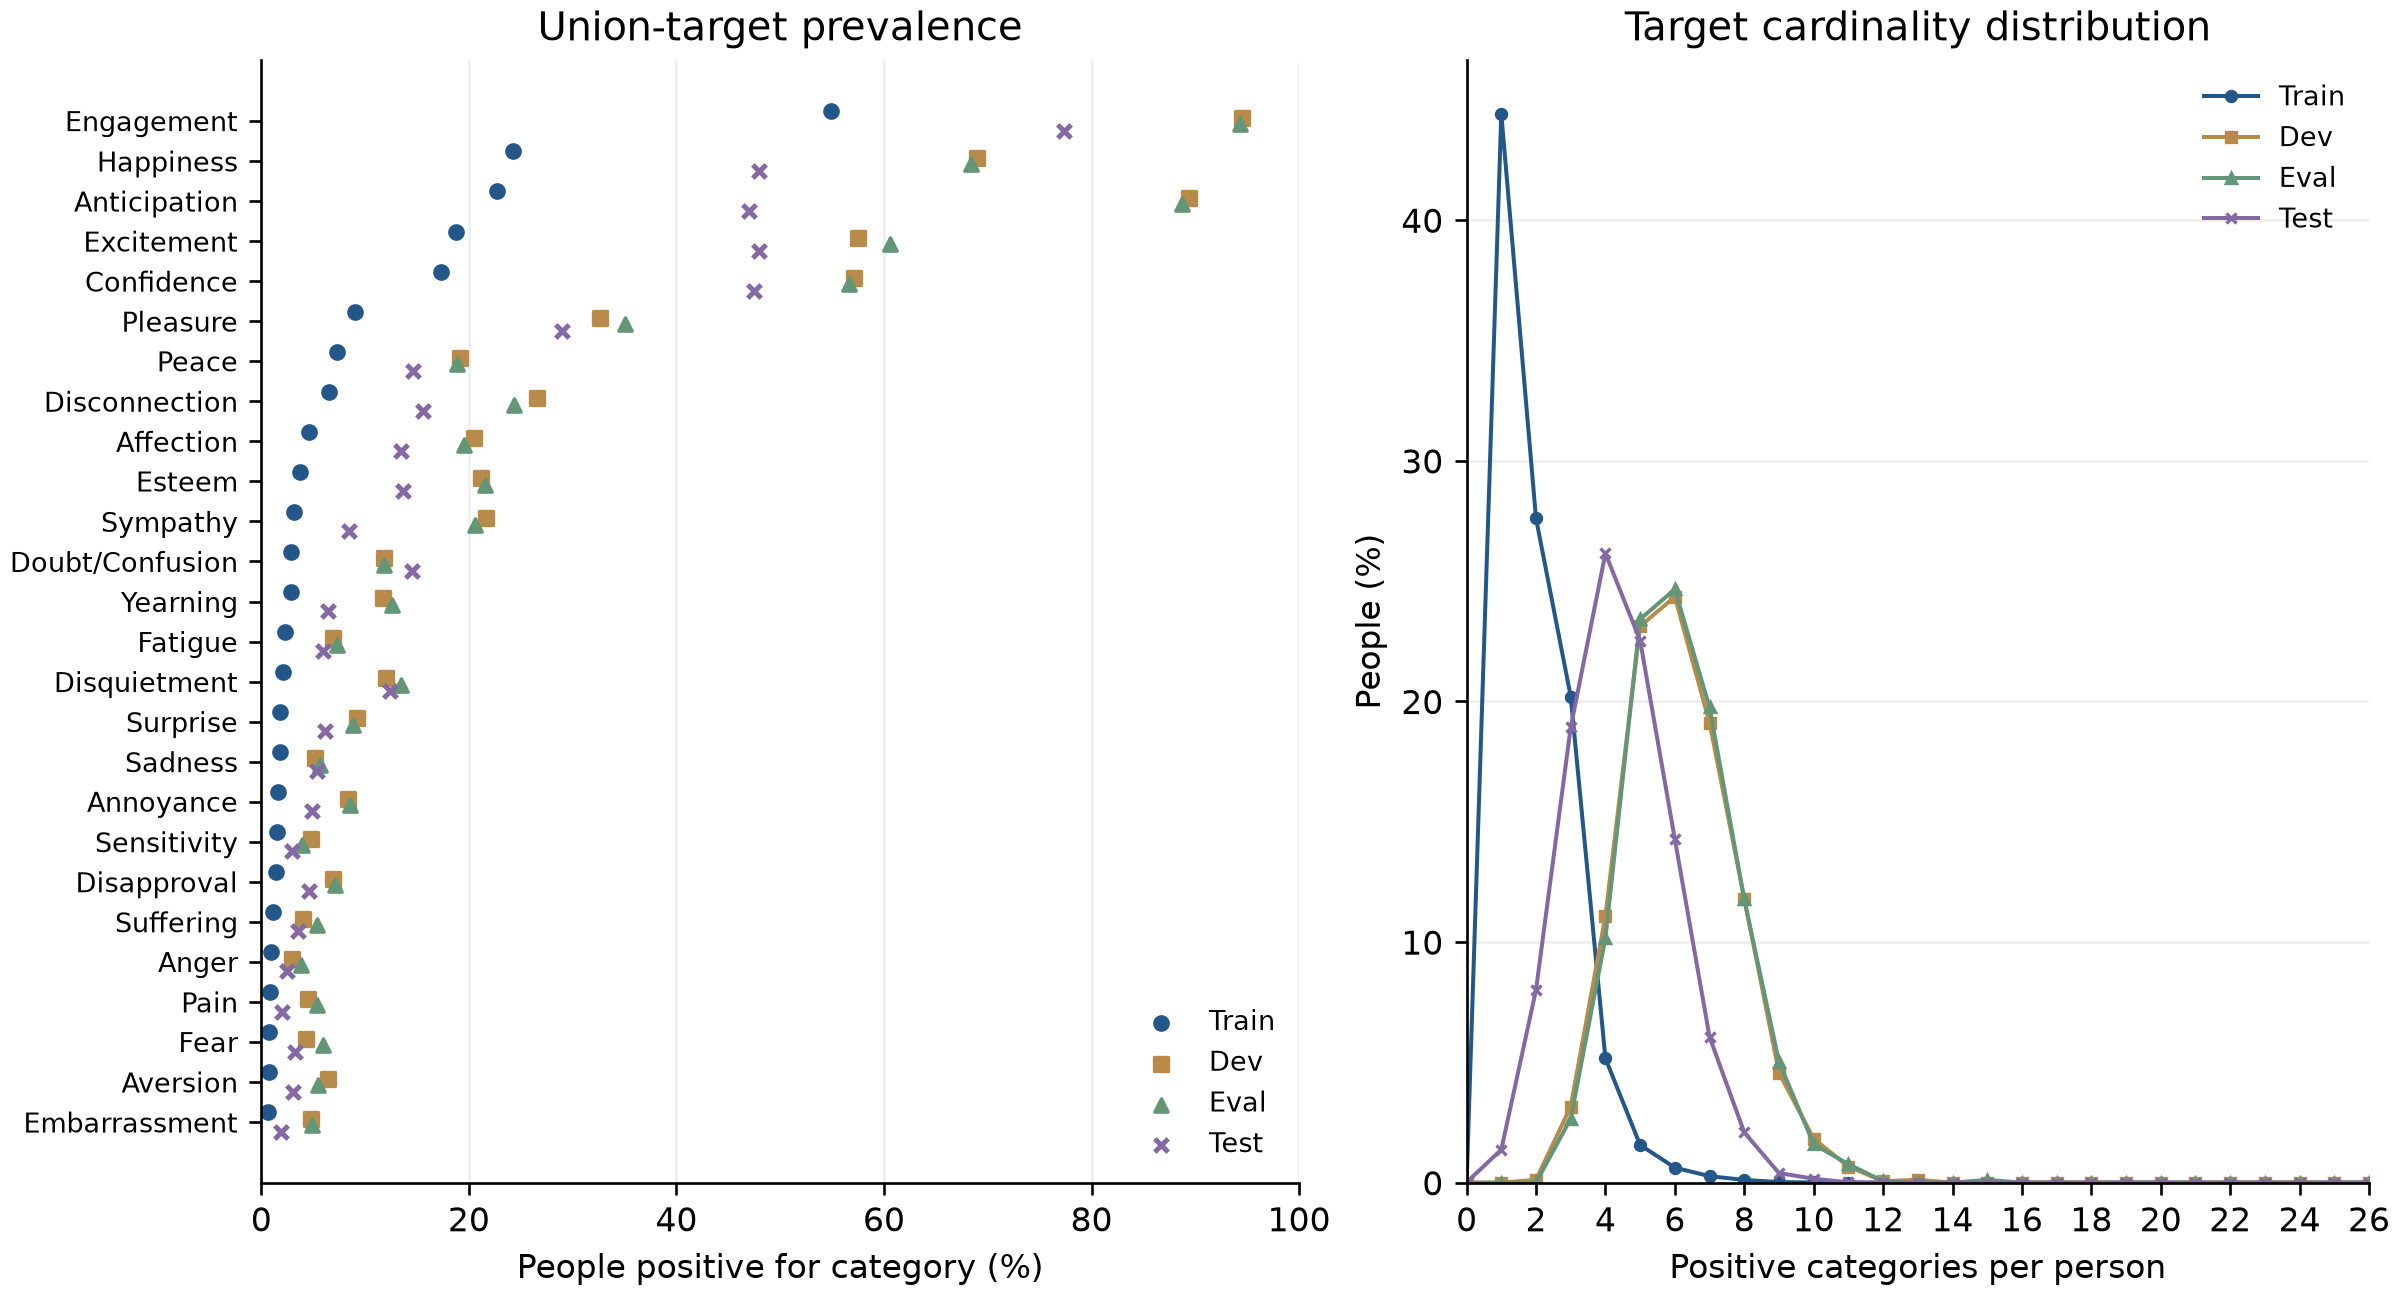
\includegraphics[width=\textwidth]{figures/data_eda.png}
\caption{Mô tả khám phá nhãn đích theo phép hợp trên các phần PAMI đã cố định. Trái: tỷ lệ người mang từng loại cảm xúc, sắp theo số mẫu dương trong train. Phải: phân phối số loại cảm xúc dương trên mỗi người. Các mô tả test được thực hiện sau đánh giá và không được dùng để lựa chọn.}
\label{fig:data}
\end{figure*}

Mật độ nhãn đích từ chú thích khác biệt rõ giữa các phần dữ liệu (Bảng~\ref{tab:data}). Phép hợp kết hợp các bản ghi chú thích loại cảm xúc hiện có; trung vị số bản ghi cũng khác nhau giữa các phần. Các bản ghi này không nhất thiết tương ứng với những người gán nhãn độc lập; cả số bản ghi lẫn phân phối biên của nhãn đều không xác lập mức đồng thuận hay độ tin cậy của chú thích. Test có \ev{eda-test-empty-targets}{1} người mang nhãn đích theo phép hợp rỗng; người này vẫn được giữ trong thống kê mô tả và lần đánh giá đã cố định. Chênh lệch số nhãn trên mỗi người và tỷ lệ xuất hiện giúp đặt khoảng cách eval--test vào bối cảnh, nhưng không xác định nguyên nhân hay định lượng đóng góp của dịch chuyển phân phối nhãn. Việc nhiều người cùng thuộc một ảnh là cơ sở để giữ nguyên nhóm ảnh khi chia validation và lấy mẫu lại theo ảnh để ước lượng độ bất định, thay vì giả định các mẫu người độc lập.

\subsection{Quy trình thực nghiệm đã cố định}\label{sec:protocol}
Trong toàn bài, eval là phần validation giữ lại để đánh giá. Checkpoint, ngưỡng, baseline nhãn hằng số và trọng số late fusion đều được chọn trên dữ liệu phát triển trước khi đánh giá. Test được chấm một lần cho các phương án đã cố định; điểm test không phải cơ sở để chọn cấu hình thay thế.

Chất lượng xếp hạng được đo bằng mAP; dự đoán sau áp dụng ngưỡng được đánh giá bằng \mf{} và \mi{}. AP được lấy trung bình trên các loại có mẫu dương. Điểm F macro được lấy trung bình trên toàn bộ các cột được cung cấp, với phép chia không xác định được quy về không. Nếu không nói khác, điểm sau áp dụng ngưỡng dùng lưới mở rộng. Trung bình và độ lệch chuẩn tổng thể của các biến thể tổng hợp các seed 42--44. Độ lệch chuẩn trên 3 seed không phải khoảng tin cậy cho hiệu năng kỳ vọng khi huấn luyện lại.

Khoảng bootstrap ghép cặp được tính bằng cách lấy mẫu lại nguyên ảnh, giữ mọi người thuộc từng ảnh, với \ev{resamples}{2000} lần lấy mẫu và mức bao phủ danh nghĩa \ev{confidence}{95}\%. Mỗi seed được so sánh riêng; các khoảng có điều kiện trên mô hình đã huấn luyện và ngưỡng cố định, đồng thời không hiệu chỉnh cho nhiều phép so sánh. Một bước so sánh riêng tính lại toàn bộ 90 bộ metric eval đã lưu của các mô hình đa phương thức và ResNet từ dự đoán đã lưu, khớp trong sai số $10^{-9}$, trước khi chạy các phân tích chỉ trên eval. Tái lập toàn bộ chuỗi xử lý còn cần dữ liệu ảnh, bộ mã hóa tiền huấn luyện, checkpoint đã huấn luyện và đặc trưng đã lưu đệm hoặc việc tạo lại các đặc trưng đó.

Lời giải thích dùng một checkpoint đầy đủ duy nhất ở seed 42. mAP của checkpoint này trên eval/test là 39.90/30.49 và \mf{} là 42.69/34.11. Chất lượng giải thích không phải trung bình trên các seed của bộ phân loại.

\begin{table*}[t]
\centering
\caption{Các biến thể đã cố định: trung bình $\pm$ độ lệch chuẩn tổng thể trên các seed 42--44. Điểm số tính theo phần trăm. Eval là phần validation giữ lại để đánh giá; xóa từ chỉ loại một tập từ cố định, không loại toàn bộ thông tin cảm xúc.}
\label{tab:variants}
\small
\tablegap
\begin{tabular}{lrrrrr}
\toprule
Biến thể & mAP eval & \mf{} eval & mAP test & \mf{} test & \mi{} test \\
\midrule
Đầy đủ & 40.06 $\pm$ 0.30 & 43.49 $\pm$ 0.59 & 30.10 $\pm$ 0.32 & 33.90 $\pm$ 0.24 & 48.80 $\pm$ 0.44 \\
ViT-only & 37.67 $\pm$ 0.68 & 40.69 $\pm$ 0.60 & 27.15 $\pm$ 0.30 & 31.59 $\pm$ 0.22 & 48.13 $\pm$ 1.16 \\
Bỏ ảnh người & 40.17 $\pm$ 0.51 & 43.34 $\pm$ 0.65 & 30.21 $\pm$ 0.15 & 33.62 $\pm$ 0.16 & 48.77 $\pm$ 0.84 \\
Bỏ ảnh ngữ cảnh & 40.37 $\pm$ 0.40 & 43.22 $\pm$ 0.50 & 30.10 $\pm$ 0.35 & 33.46 $\pm$ 0.25 & 47.94 $\pm$ 0.86 \\
Bỏ dấu hiệu người & 39.99 $\pm$ 0.16 & 42.22 $\pm$ 0.32 & 28.49 $\pm$ 0.05 & 32.19 $\pm$ 0.11 & 49.37 $\pm$ 0.79 \\
Bỏ dấu hiệu ngữ cảnh & 40.82 $\pm$ 0.16 & 43.70 $\pm$ 0.75 & 30.28 $\pm$ 0.27 & 33.85 $\pm$ 0.36 & 49.40 $\pm$ 0.53 \\
Xóa từ & 40.40 $\pm$ 0.32 & 43.41 $\pm$ 0.36 & 29.97 $\pm$ 0.27 & 33.41 $\pm$ 0.42 & 48.96 $\pm$ 0.42 \\
\bottomrule
\end{tabular}
\end{table*}

\subsection{Dự đoán và ablation có huấn luyện lại}\label{sec:prediction}
Bỏ token ngữ nghĩa gây mức giảm lớn nhất và nhất quán nhất (Bảng~\ref{tab:variants}, Hình~\ref{fig:prediction}): ViT-only là biến thể thấp nhất trên cả eval và test, và trên test mô hình đầy đủ vượt nó khoảng 3 điểm mAP, với khoảng không chứa giá trị không ở cả ba seed (Bảng~\ref{tab:bootstrap}). Che dấu hiệu về người là mức giảm nhất quán thứ hai: mAP test giảm còn 28.49, và chênh lệch giữa mô hình đầy đủ với no-person-cues không chứa giá trị không ở mọi seed trên cả hai thước đo. Như vậy, dấu hiệu văn bản, đặc biệt là dấu hiệu về người, mang thông tin dự đoán mà đặc trưng ViT đóng băng không cung cấp.

Các ablation còn lại cho kết quả sát mô hình đầy đủ. Đặt ảnh người, ảnh ngữ cảnh về không hoặc bỏ dấu hiệu ngữ cảnh làm mAP test trung bình thay đổi dưới 0.2 điểm; các khoảng theo từng seed phần lớn chứa giá trị không hoặc đổi dấu giữa các seed. Trên eval, no-context-cues có mAP trung bình cao nhất (40.82). Do đó, dấu hiệu ngữ cảnh chưa cho thấy lợi ích đáng tin cậy trong biểu diễn này, và các luồng thị giác chồng lấp với nhau cũng như với văn bản.

Biến thể xóa từ làm mAP test trung bình thay đổi từ 30.10 xuống 29.97. Chênh lệch giữa mô hình đầy đủ và biến thể xóa từ chứa giá trị không về mAP ở mọi seed, còn các chênh lệch \mf{} nhỏ không chứa giá trị không ở seed 43 và 44. Bộ phân loại vì vậy không phụ thuộc vào việc VLM viết tên cảm xúc vào dấu hiệu. Kết quả này không chứng minh rằng ngữ nghĩa cảm xúc đã bị loại bỏ, rằng cấu trúc đồ thị mang lại lợi ích, hay rằng prompt suy luận chuỗi gây ra lợi ích dự đoán.

\begin{figure*}[t]
\centering
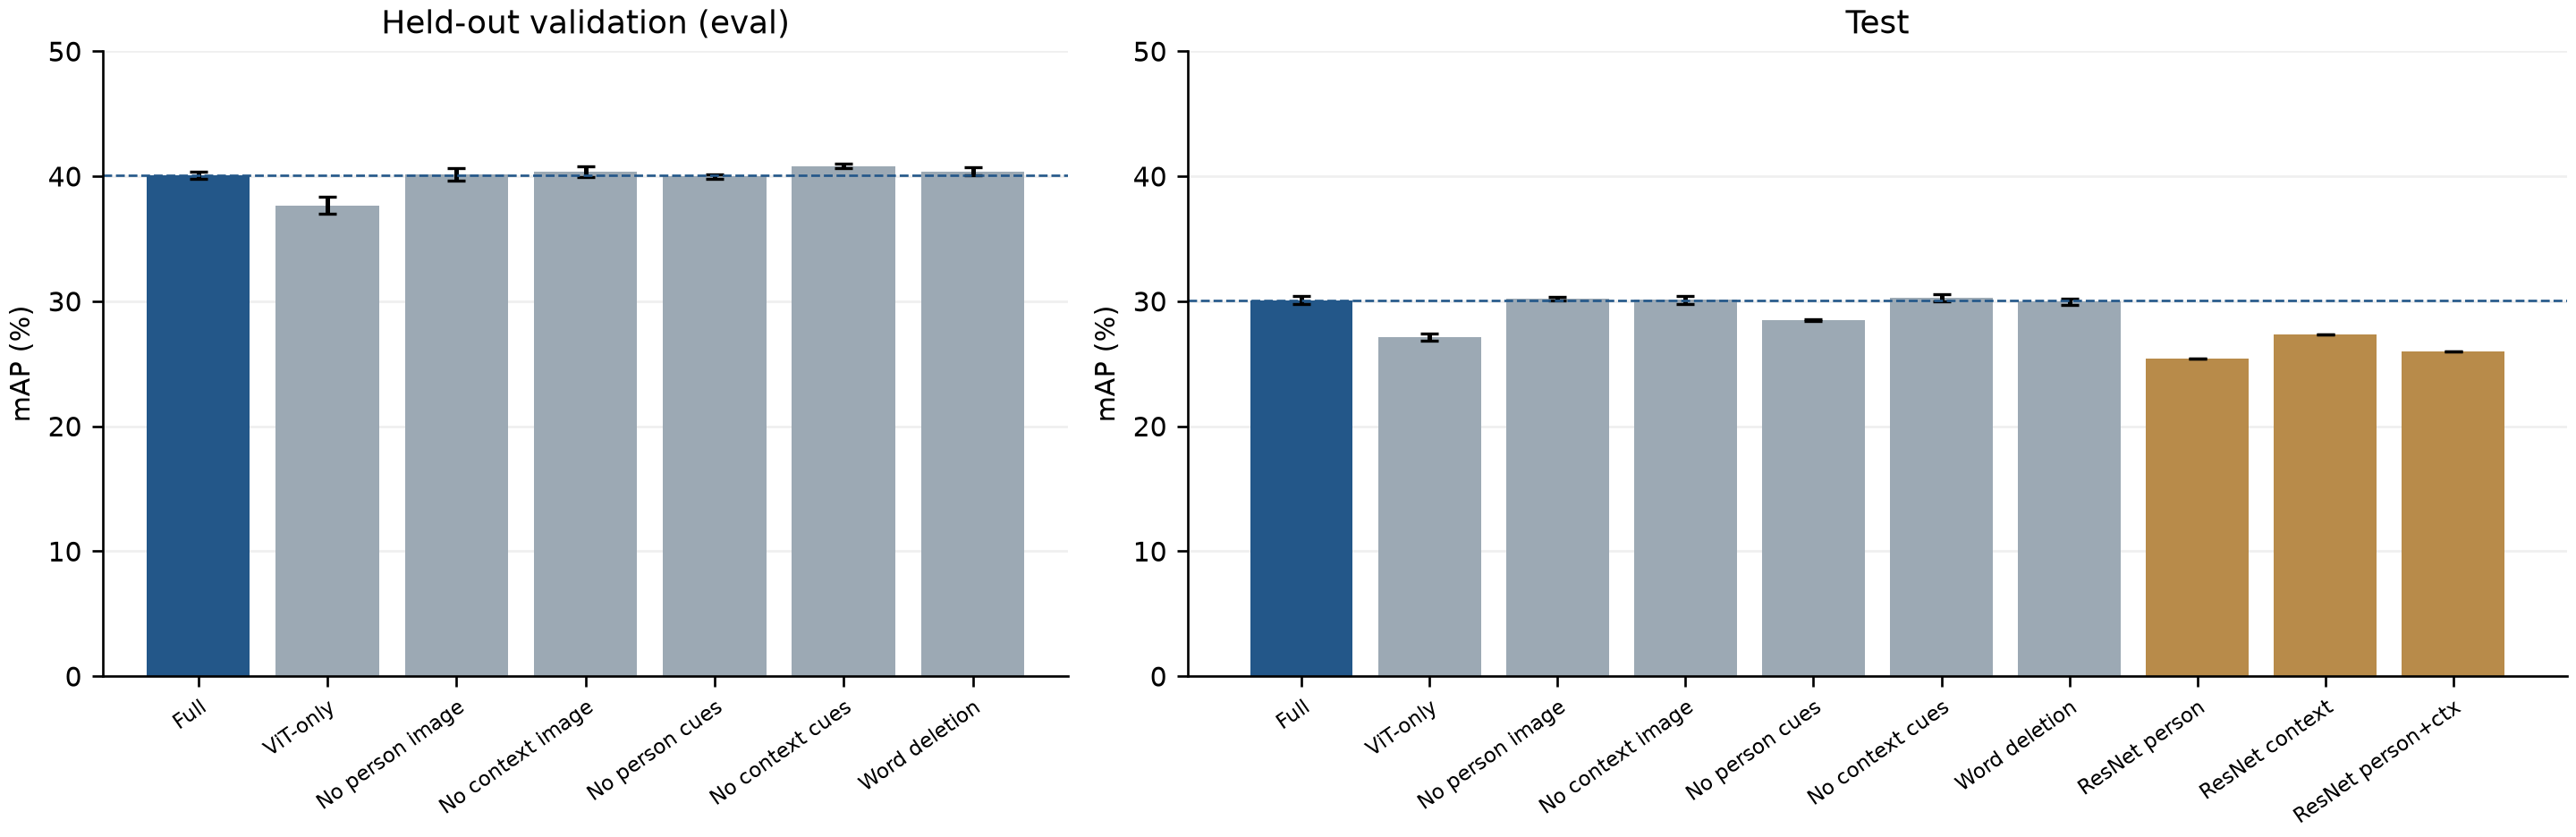
\includegraphics[width=\textwidth]{figures/prediction.png}
\caption{mAP của các biến thể đã cố định và, trên test, của các baseline ResNet-50 được huấn luyện. Thanh sai số là độ lệch chuẩn tổng thể giữa các seed huấn luyện, không phải khoảng tin cậy bootstrap; baseline ResNet chỉ có một seed. Đường gạch đánh dấu mô hình đầy đủ.}
\label{fig:prediction}
\end{figure*}

\begin{table*}[t]
\centering
\caption{Chênh lệch trên test từ bootstrap ghép cặp theo ảnh (đầy đủ trừ B), tính bằng điểm phần trăm, ở seed 42, kèm số seed (trên 3) có khoảng danh nghĩa 95\% không chứa giá trị không. Các khoảng có điều kiện trên mô hình đã huấn luyện và không bao gồm độ bất định do huấn luyện lại.}
\label{tab:bootstrap}
\small
\begin{tabular}{lrrrr}
\toprule
B & $\Delta$ mAP [KTC 95\%] & Seed & $\Delta$ \mf{} [KTC 95\%] & Seed \\
\midrule
ViT-only & +2.96 [2.49, 3.49] & 3/3 & +2.64 [2.08, 3.23] & 3/3 \\
Bỏ ảnh người & +0.14 [$-$0.28, 0.56] & 0/3 & +0.30 [$-$0.15, 0.71] & 0/3 \\
Bỏ ảnh ngữ cảnh & +0.78 [0.13, 1.49] & 2/3 & +0.96 [0.27, 1.65] & 1/3 \\
Bỏ dấu hiệu người & +2.06 [1.41, 2.67] & 3/3 & +1.80 [1.28, 2.29] & 3/3 \\
Bỏ dấu hiệu ngữ cảnh & $-$0.12 [$-$0.47, 0.20] & 1/3 & $-$0.17 [$-$0.57, 0.24] & 1/3 \\
Xóa từ & +0.16 [$-$0.16, 0.47] & 0/3 & +0.16 [$-$0.21, 0.50] & 2/3 \\
ResNet người & +5.10 [4.31, 5.98] & 3/3 & +11.04 [10.01, 11.99] & 3/3 \\
ResNet ngữ cảnh & +3.15 [2.13, 4.06] & 3/3 & +3.18 [2.25, 4.14] & 3/3 \\
ResNet người + ngữ cảnh & +4.52 [3.79, 5.36] & 3/3 & +13.32 [12.37, 14.26] & 3/3 \\
Nhãn hằng số & --- & --- & +8.99 [8.11, 9.77] & 3/3 \\
\bottomrule
\end{tabular}
\end{table*}

Với no-context-image, khoảng mAP ở seed 42 không chứa giá trị không và nghiêng về mô hình đầy đủ, nhưng khoảng ở seed 44 không chứa giá trị không theo chiều ngược lại; với no-context-cues, khoảng \mf{} ở seed 43 nghiêng về mô hình đầy đủ, còn khoảng mAP ở seed 44 nghiêng về ablation. Vì các kết quả trái chiều này, chúng tôi xem các ablation đó là không khác biệt đáng tin cậy, thay vì xem là lợi ích hay tổn thất.

\subsection{Baseline thị giác và khả năng bám theo mục tiêu}\label{sec:baselines}
Các baseline thị giác dùng \ev{resnet}{ResNet-50} tiền huấn luyện trên ImageNet \cite{resnet}: chỉ người, chỉ ngữ cảnh từ ảnh toàn cảnh và nối đặc trưng từ bộ mã hóa người/ngữ cảnh. Chúng được huấn luyện \ev{resnet-epochs}{30} epoch với đầu vào vuông cạnh \ev{resnet-image}{224} pixel và phần đệm ảnh cắt \ev{crop-padding}{5}\%. Khác với ViT đóng băng, backbone của chúng được huấn luyện. Đây là các hệ thống hoàn chỉnh dùng để so sánh, không phải ước lượng có kiểm soát về đóng góp của văn bản. Mỗi baseline chỉ có một seed huấn luyện, và checkpoint được chọn trên toàn bộ validation, gồm cả eval.

\begin{table}[t]
\centering
\caption{Baseline ResNet với một lần chạy. mAP validation là giá trị lớn nhất trong nhật ký huấn luyện; test dùng ngưỡng chọn từ validation. Điểm số tính theo phần trăm.}
\label{tab:resnet}
\small
\tablegap
\begin{tabular}{lrrr}
\toprule
Đầu vào & mAP val & mAP test & \mf{} test \\
\midrule
Người & \ev{resnet-person_only-val-map}{39.45} & \ev{resnet-person_only-test-map}{25.39} & \ev{resnet-person_only-test-macro_f1}{23.07} \\
Ngữ cảnh & \ev{resnet-context_only-val-map}{37.87} & \ev{resnet-context_only-test-map}{27.35} & \ev{resnet-context_only-test-macro_f1}{30.94} \\
Người + ngữ cảnh & \ev{resnet-person_context-val-map}{40.14} & \ev{resnet-person_context-test-map}{25.97} & \ev{resnet-person_context-test-macro_f1}{20.79} \\
\bottomrule
\end{tabular}
\end{table}

Bảng~\ref{tab:resnet} cho thấy thứ hạng thay đổi từ validation sang test: mô hình kết hợp có mAP validation tốt nhất cao nhất, nhưng context-only dẫn đầu về mAP và \mf{} trên test. Context-only vẫn nhìn thấy mục tiêu trong ảnh toàn cảnh. Trên test, mô hình đa phương thức đầy đủ vượt cả ba baseline ResNet trên cả hai thước đo, với khoảng không chứa giá trị không ở mọi seed (Bảng~\ref{tab:bootstrap}); so với baseline mạnh nhất là context-only, chênh lệch ở seed 42 là +3.15 điểm mAP và +3.18 điểm \mf{}. Các khoảng này không ước lượng biến thiên do huấn luyện lại ResNet.

Baseline hằng số chọn \ev{constant-k}{26} nhãn, tức dự đoán mọi loại cảm xúc cho mọi người trong test. mAP, \mf{} và \mi{} trên test lần lượt là \ev{constant-test-map}{16.98}, \ev{constant-test-macro_f1}{25.12} và \ev{constant-test-micro_f1}{29.03}. AP của cách xếp hạng hằng số rút về tỷ lệ xuất hiện của từng loại. Chọn số nhãn hằng số bằng điểm F macro ưu tiên thêm những loại có mẫu dương; vượt baseline này là kết quả kiểm tra tính hợp lý cơ bản, không phải bằng chứng mạnh cho suy luận theo ngữ cảnh.

Đầu ra đã lưu của notebook baseline thị giác cung cấp các phép chẩn đoán khả năng bám theo mục tiêu cho ResNet kết hợp. Đặt luồng người về không và che mục tiêu trong ảnh toàn cảnh cho mAP test \ev{region-delta_person-map}{20.35}; che nền nhưng giữ vùng mục tiêu cho \ev{region-delta_context-map}{24.71}. Đặt luồng người về không và che ngẫu nhiên một vùng có cùng kích thước cho \ev{region-delta_random-map}{20.95}, so với mAP nguyên trạng \ev{resnet-person_context-test-map}{25.97}. Các kết quả này không có khoảng bất định đã lưu. Điều kiện ngẫu nhiên không chỉ che ngẫu nhiên, và thí nghiệm không đánh giá mức bám sát bằng chứng của văn bản đa phương thức.

Trong phép hoán đổi mục tiêu, ảnh được giữ nguyên còn ảnh cắt của một người được chú thích khác thay cho ảnh cắt người ban đầu. Dự đoán có điểm F theo mẫu cho mục tiêu mới cao hơn điểm F cho người ban đầu ở \ev{swap-swap_accuracy}{40.47}\% trên tổng số \ev{swap-num_pairs}{9988} cặp có hướng từ \ev{swap-num_images}{1783} ảnh; các trường hợp bằng điểm không được tính là cao hơn. Các trường hợp bằng điểm chiếm \ev{swap-tie_rate}{22.97}\%, và trung bình điểm F của mục tiêu mới trừ người ban đầu là \ev{swap-mean_target_minus_source_f1}{0.01405}. Đây là phép chẩn đoán khả năng bám theo mục tiêu, không phải độ chính xác nhận diện hay phép kiểm định so với mức ngẫu nhiên đã hiệu chuẩn. Nhãn chồng lấp và việc xem các trường hợp bằng điểm là thất bại hạn chế cách diễn giải kết quả.

\subsection{So sánh trên eval với ResNet và late fusion}\label{sec:eval}
Một bước so sánh riêng chạy trên CPU đánh giá dự đoán đã lưu của 1691 người trong eval (Bảng~\ref{tab:eval}). Ensemble, late fusion và phân tích theo nhóm là các phân tích sau, chỉ trên eval: ensemble lấy trung bình ba seed của mô hình đầy đủ, late fusion là $w\cdot\text{ensemble}+(1-w)\cdot\text{ResNet người+ngữ cảnh}$, còn $w=0.5$ và mọi ngưỡng được cố định trên dev (mAP dev 40.34 khi chỉ dùng ResNet, 41.54 khi chỉ dùng ensemble, 44.79 khi trộn). Không tổ hợp nào trong số này được chấm trên test.

\begin{table}[t]
\centering
\caption{Kết quả trên eval (validation giữ lại) từ dự đoán đã lưu, lưới ngưỡng mở rộng. Đầy đủ và ViT-only là trung bình ba seed. Ensemble lấy trung bình ba seed đầy đủ; late fusion trộn ensemble với ResNet người + ngữ cảnh. Hai dòng này là phân tích sau, chỉ trên eval. Điểm số tính theo phần trăm.}
\label{tab:eval}
\small
\tablegap
\begin{tabular}{lrr}
\toprule
Mô hình & mAP & \mf{} \\
\midrule
Đầy đủ (3 seed) & 40.06 & 43.49 \\
ViT-only (3 seed) & 37.67 & 40.69 \\
Ensemble & 41.32 & 44.18 \\
Late fusion ($w=0.5$) & 45.38 & 45.08 \\
\midrule
ResNet người & 40.30 & 40.33 \\
ResNet ngữ cảnh & 38.73 & 41.39 \\
ResNet người + ngữ cảnh & 40.61 & 39.57 \\
Hằng số ($k=26$) & 23.78 & 32.60 \\
\bottomrule
\end{tabular}
\end{table}

Trên eval, mô hình đầy đủ ngang các baseline ResNet về mAP nhưng cao hơn về \mf{}. So với ResNet người + ngữ cảnh, khoảng mAP của mô hình đầy đủ chứa giá trị không ở cả ba seed, còn chênh lệch \mf{} (+3.12 đến +4.54 điểm) không chứa giá trị không ở mọi seed. Checkpoint ResNet được chọn trên phần validation có chứa eval, nên điểm eval của chúng có thể lạc quan; so sánh trên test không bị ảnh hưởng. Late fusion cho mức tăng lớn nhất trên eval so với ResNet người + ngữ cảnh, +4.77 mAP [3.59, 6.42] và +5.51 \mf{} [3.80, 7.27], cho thấy hai họ mô hình mắc lỗi bổ trợ nhau một phần. Dùng fusion trên test sẽ là một cấu hình mới.

Chênh lệch AP theo từng loại giữa trung bình mô hình đầy đủ và ResNet người + ngữ cảnh dương ở 12 trên 26 loại, lớn nhất ở Annoyance (+6.5), Affection (+4.7) và Disapproval (+4.4), âm nhiều nhất ở Peace ($-$9.0), Disconnection ($-$8.0) và Doubt/Confusion ($-$7.0). Khi nhóm theo số người được chú thích trong ảnh, mô hình đầy đủ vượt ResNet người + ngữ cảnh ở ảnh có một người (44.2 so với 42.7 mAP) hoặc hai người (38.8 so với 36.2), nhưng kém ở ảnh có ba hoặc bốn người (37.1 so với 42.1, 127 ảnh). Dấu hiệu và đồ thị ngữ nghĩa có thể trộn thông tin giữa những người trong ảnh đông người. Nhóm từ năm người trở lên chỉ có 23 ảnh.

\subsection{Kết quả giải thích}\label{sec:explanations}
Checkpoint ở seed 42 tạo ra 1671 phản hồi dùng được từ 1691 người trong eval và 7184 phản hồi dùng được từ 7280 người trong test. Do đó, các thước đo trên phản hồi dùng được loại 20 đầu ra eval và 96 đầu ra test, thay vì xem mọi phản hồi được sinh ra là thành công; 1.12\% phản hồi eval và 1.26\% phản hồi test bị cắt cụt.

\begin{table}[t]
\centering
\caption{Chẩn đoán lời giải thích từ một checkpoint. Các tỷ lệ dùng phản hồi dùng được, riêng phép đối chiếu con số dùng các lượt trích số đã trích xuất.}
\label{tab:explanations}
\small
\tablegap
\begin{tabular}{lrr}
\toprule
Chỉ tiêu & Eval & Test \\
\midrule
\multicolumn{3}{l}{\emph{Phương thức được nêu (số phản hồi)}} \\
\quad Người & 1664 & 7149 \\
\quad Ngữ cảnh & 7 & 35 \\
\quad Đồ thị & 0 & 0 \\
\multicolumn{3}{l}{\emph{Phương thức giảm nhiều nhất (số phản hồi)}} \\
\quad Người & 476 & 2268 \\
\quad Ngữ cảnh & 900 & 3664 \\
\quad Đồ thị & 295 & 1252 \\
\midrule
Khớp phương thức (\%) & 28.61 & 31.83 \\
Khớp hằng số (\%) & 53.86 & 51.00 \\
Con số khớp (\%) & 99.99 & 99.92 \\
Số lượt trích số & 8086 & 35101 \\
Nhắc nhãn ngoài dự đoán (\%) & 0.48 & 0.88 \\
\bottomrule
\end{tabular}
\end{table}

Bảng~\ref{tab:explanations} cho thấy xu hướng rất mạnh về việc nêu phương thức người; phương thức đồ thị không bao giờ được nêu. Phương thức mà khi bỏ đi làm giảm điểm các nhãn dự đoán nhiều nhất thường là ngữ cảnh (900 trên 1671 phản hồi eval và 3664 trên 7184 phản hồi test), nên lời giải thích gần như luôn nêu người chỉ khớp với phương thức đo được ở 28.61\% và 31.83\% trường hợp. Mốc tham chiếu hằng số luôn nêu ngữ cảnh đạt 53.86\% và 51.00\%. Như vậy, lời giải thích không xác định được phương thức mà bộ phân loại nhạy nhất.

\begin{table*}[t]
\centering
\caption{Chẩn đoán can thiệp token trên lời giải thích dùng được của checkpoint chính. Comp.: comprehensiveness (lớn hơn được ưu tiên); suff.: độ chênh sufficiency (nhỏ hơn được ưu tiên). Đây không phải điểm đánh giá mức bám sát bằng chứng của văn bản tự do.}
\label{tab:interventions}
\small
\begin{tabular}{lrrrr}
\toprule
Quy tắc chọn & Comp. eval & Suff. eval & Comp. test & Suff. test \\
\midrule
Phương thức được nêu & 0.0207 & 0.0624 & 0.0213 & 0.0612 \\
Phương thức đo thường gặp nhất & 0.0453 & 0.0356 & 0.0441 & 0.0364 \\
Trung bình với trọng số bằng nhau & 0.0281 & 0.0583 & 0.0283 & 0.0577 \\
Phương thức đo có mức giảm lớn nhất & 0.0649 & 0.0158 & 0.0655 & 0.0149 \\
\bottomrule
\end{tabular}
\end{table*}

Phương thức được nêu kém mốc tham chiếu trung bình với trọng số bằng nhau về cả comprehensiveness lẫn sufficiency, và kém mốc tham chiếu hằng số với khoảng cách lớn hơn (Bảng~\ref{tab:interventions}, Hình~\ref{fig:faithfulness}). Chọn phương thức có mức giảm lớn nhất theo phép đo cho comprehensiveness cao hơn nhiều và độ chênh sufficiency nhỏ hơn. Lợi thế comprehensiveness của cách chọn này là điều được kỳ vọng ngay từ định nghĩa. So sánh cho thấy khoảng cách giữa lựa chọn trong lời giải thích và phép chẩn đoán, không phải một benchmark lời giải thích của con người.

Mức khớp con số cao có ý nghĩa hẹp hơn tính đúng đắn về thực tế: một con số được phép có thể đi kèm mô tả sai về cảm xúc, phương thức hoặc chiều thay đổi. Tỷ lệ nhắc nhãn ngoài dự đoán thấp chỉ bao quát tên nhãn đúng nguyên văn. Không có đánh giá của con người về mức bám sát bằng chứng, tính hữu ích hay tính đúng đắn về tâm lý. Bằng chứng cho thấy hệ thống diễn đạt con số theo các ràng buộc đã đặt ra nhưng không phân biệt được phương thức; bằng chứng này chưa xác lập rằng lời giải thích phản ánh trung thực suy luận của bộ phân loại.

\begin{figure*}[t]
\centering
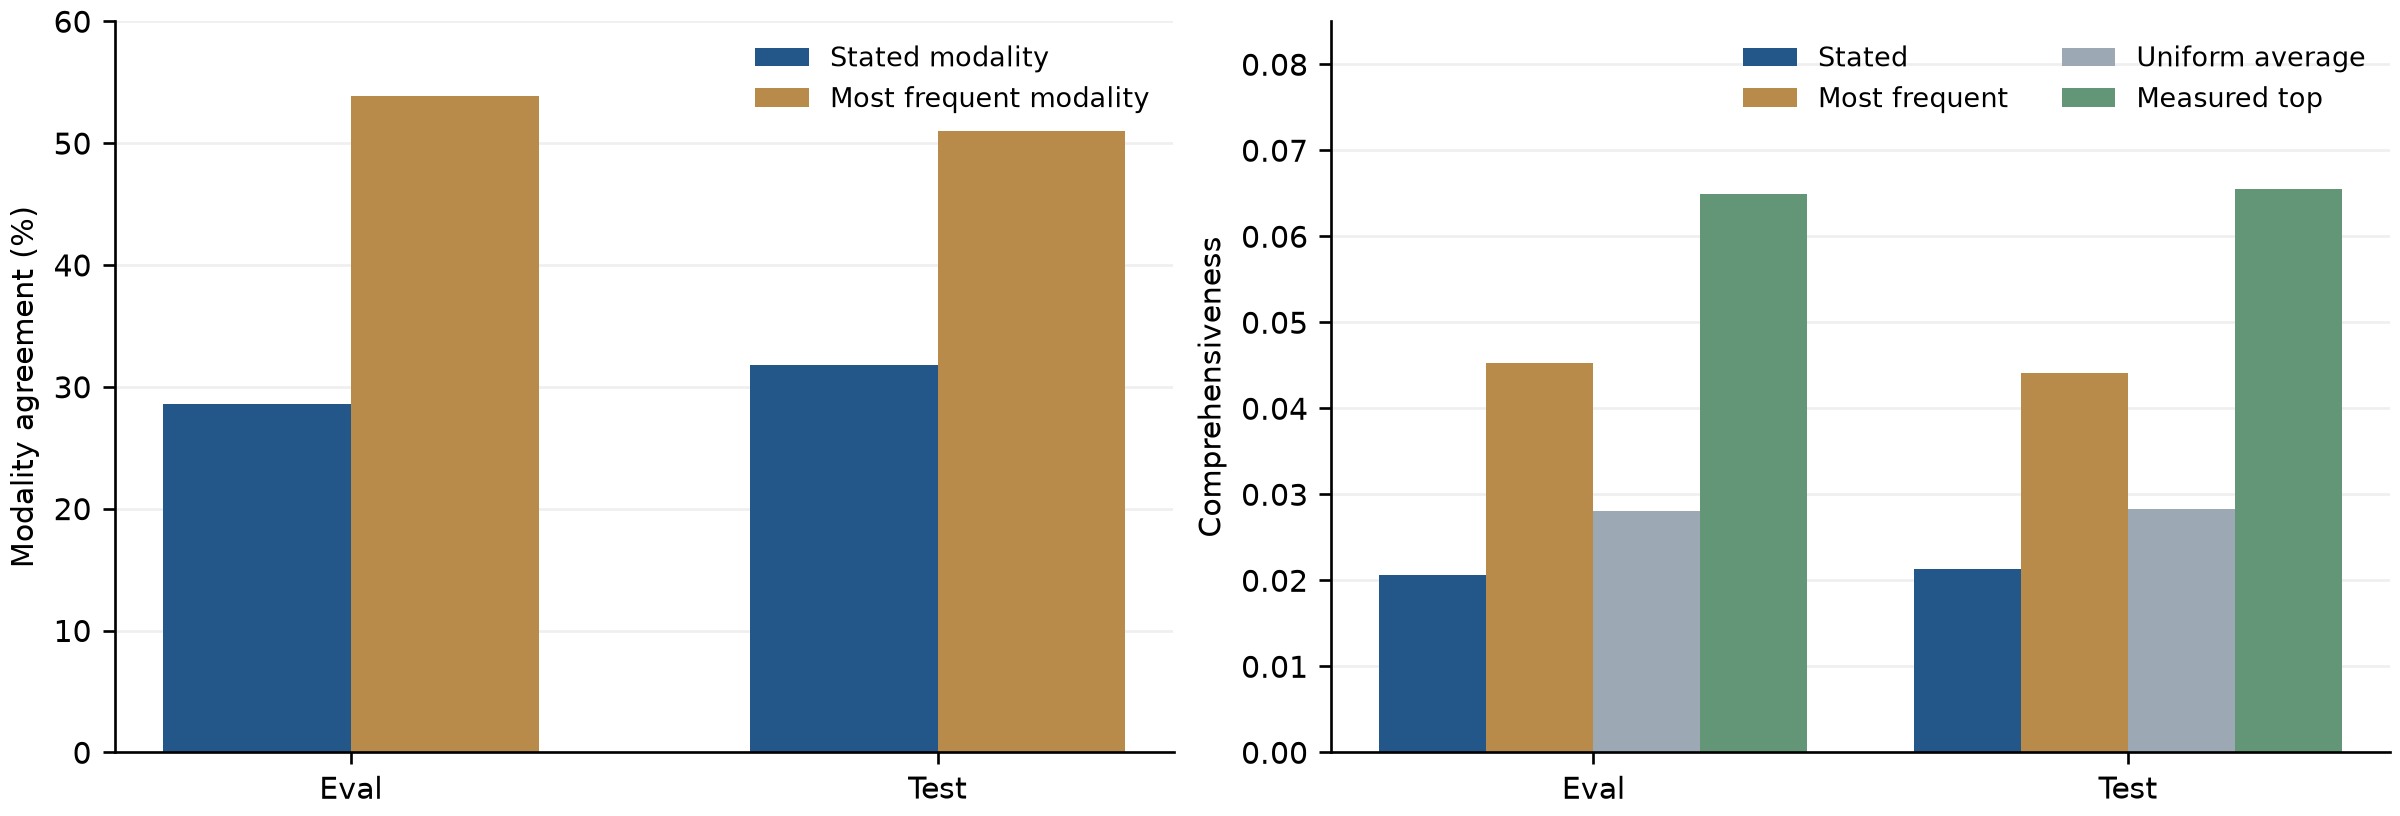
\includegraphics[width=\textwidth]{figures/faithfulness.png}
\caption{Mức khớp và comprehensiveness của lời giải thích ở seed 42. Mốc tham chiếu hằng số dùng phương thức xuất hiện thường xuyên nhất theo phép đo trên từng phần dữ liệu; mốc tham chiếu mức giảm lớn nhất được suy ra trực tiếp từ tiêu chí can thiệp.}
\label{fig:faithfulness}
\end{figure*}

\subsection{Thảo luận và hạn chế}\label{sec:discussion}
Lợi ích dự đoán và tính trung thực của lời giải thích trả lời những câu hỏi khác nhau. Văn bản cải thiện nhận diện so với biểu diễn thị giác đóng băng tương ứng và so với các baseline ResNet-50 được huấn luyện, nhưng lời giải thích bằng lời không xác định được luồng thông tin quan trọng. Ngược lại, khớp với can thiệp chưa đủ để khẳng định dấu hiệu thực sự nhìn thấy được hay cảm xúc suy ra là đúng về tâm lý. Chuỗi xử lý theo giai đoạn là cách tổ chức thông tin có thể kiểm tra được, không phải mô hình suy luận cảm xúc của con người đã được kiểm chứng.

Biến thể đầy đủ dự đoán trung bình 10.25 nhãn trên mỗi người trong test khi lấy trung bình qua các seed. So với số nhãn đích quan sát được trong Bảng~\ref{tab:data}, kết quả cho thấy khác biệt giữa kích thước tập nhãn dự đoán và tập nhãn quan sát khi dùng ngưỡng dev cố định. EDA cũng cho thấy mật độ nhãn đích và tần suất loại cảm xúc không đồng đều giữa các phần dữ liệu. Các mô tả này không tách riêng được nguyên nhân suy giảm hiệu năng từ eval sang test; mức đồng thuận chú thích và độ tin cậy của biểu quyết vẫn chưa được đo.

Bước trích xuất dấu hiệu phân tích cú pháp thành công \ev{cue-parse_rate}{100.00}\% bản ghi train/validation và đạt phép kiểm tra cấu trúc ở \ev{cue-schema_rate}{99.65}\%; các tỷ lệ trên test là \ev{test-cue-parse_rate}{99.99}\% và \ev{test-cue-schema_rate}{99.63}\%. Chúng mô tả cấu trúc, không phản ánh mức đúng của nội dung nhìn thấy được. Thời gian xử lý theo batch được ghi nhận là \ev{batch-16-seconds}{0.838}, \ev{batch-32-seconds}{0.269} và \ev{batch-48-seconds}{0.217} giây/người cho các batch \ev{batch-16}{16}, \ev{batch-32}{32} và \ev{batch-48}{48}; tỷ lệ trùng khớp hoàn toàn với dấu hiệu tham chiếu đã lưu là \ev{batch-16-same}{56.25}\%, \ev{batch-32-same}{59.38}\% và \ev{batch-48-same}{58.33}\%. Khác biệt về số mẫu và điều kiện chạy không cho phép khẳng định có kiểm soát về mức tăng tốc hay tính tương đương của đầu ra.

Việc quy đóng góp vẫn bị hạn chế bởi đầu vào chồng lấp. Văn bản trộn thông tin người, ngữ cảnh và quan hệ; đặc trưng ảnh toàn cảnh chứa cả mục tiêu. Ablation token và nút không thể xác định duy nhất đóng góp của quan hệ hay định vị một vùng làm căn cứ giải thích. Mô hình giải thích nhìn ảnh một cách độc lập, thao tác đặt về không có thể tạo biểu diễn lạ, và tiêu chí mức giảm lớn nhất theo phép đo phụ thuộc vào các loại cảm xúc được dự đoán. Không có can thiệp nào xác minh ngữ nghĩa câu. Khoảng theo từng seed không hỗ trợ khẳng định về các lần huấn luyện lại nói chung, còn kết quả ResNet với một seed, có checkpoint chọn trên dữ liệu chứa eval, hạn chế so sánh giữa các họ mô hình trên eval.

Bằng chứng mạnh hơn sẽ đòi hỏi đánh giá độc lập về mức bám sát bằng chứng, can thiệp có ý nghĩa lên vùng ảnh hoặc quan hệ, một prompt giải thích bị ràng buộc nêu phương thức có mức giảm lớn nhất, và so sánh tường minh giữa trả lời trực tiếp với suy luận qua bước trung gian. Các thí nghiệm này chưa được hoàn thành. Những nghiên cứu như vậy cần dữ liệu phát triển và đánh giá mới, thay vì lựa chọn theo kết quả test hiện tại.

\section{Kết luận}\label{sec:conclusion}
Chúng tôi đánh giá một chuỗi nhận diện cảm xúc theo ngữ cảnh qua các giai đoạn, thể hiện dấu hiệu bằng văn bản, hợp nhất chúng với đặc trưng thị giác và diễn đạt bằng lời bằng chứng can thiệp của bộ phân loại. Dấu hiệu văn bản được mã hóa thành đồ thị ngữ nghĩa cải thiện nhận diện trên test so với chỉ dùng đặc trưng thị giác đóng băng và so với ba baseline ResNet-50 được huấn luyện, nhất quán qua ba seed; đóng góp đến từ toàn bộ dấu hiệu và từ dấu hiệu về người, còn dấu hiệu ngữ cảnh, từng token thị giác riêng lẻ và tên cảm xúc nguyên văn hầu như không tạo khác biệt đáng tin cậy. Trên eval, late fusion với một baseline ResNet gợi ý lỗi bổ trợ nhau, nhưng chưa được đánh giá trên test. Lời giải thích tái hiện sát các giá trị số được phép, song gần như luôn nêu luồng người và thấp hơn mốc tham chiếu phương thức hằng số. Các thí nghiệm không xác lập lợi thế của prompt suy luận chuỗi so với trả lời trực tiếp, cũng không xác lập tính trung thực của lời giải thích về mặt nhân quả hay qua đánh giá của con người.

\bibliographystyle{IEEEtran}
\bibliography{refs}
\end{document}
